\section{Method}
% In this section, we initially outline the general process of implementing Singular Value Decomposition (SVD) for weight matrix compression in LLMs, as detailed in Section \ref{sec:method-pre}. Following this, Section \ref{sec:method-challenge} identifies and discusses two major challenges associated with implementing SVD-based methods in LLMs. To address these challenges, we propose our Activation-aware Singular Value Decomposition (\asvd) and Sensitivity-aware Truncation Rank Searching (STRC) in Sections \ref{sec:method-activation} and \ref{sec:method-sensitivity}, respectively. 

\subsection{Naïve SVD for Compressing Weight Matrix}
\label{sec:method-pre}

% A large language model (LLM) is primarily based on the Transformer model~\cite{vaswani2017attention}.
% A significant amount of memory and computational overhead is incurred by Transformers' linear weight matrices, especially in its multi-head attention (MHA) and feed-forward layers~\cite{tay2022efficientsurvey}. Consequently, we focus primarily on decomposing these linear weight matrices in this paper. 
Singular Value Decomposition (SVD) can be used to decompose the weights of linear layers, which involves decomposing a weight matrix $\mathbf{W}\in \mathbb{R}^{m \times n}$ into three matrices: $\mathbf{U}$, $\mathbf{\Sigma}$, and $\mathbf{V}^T$, such that $\mathbf{W} \approx \mathbf{U} \mathbf{\Sigma} \mathbf{V}^T$), where $\mathbf{\Sigma}$ is an $m \times n$ diagonal matrix, the diagonal values in $\mathbf{\Sigma}$ are the singular values of $\mathbf{W}$, and $\mathbf{U}\in \mathbb{R}^{m \times m}$ and $\mathbf{V}\in \mathbb{R}^{n \times n}$ are corresponding right and left singular vector matrices, respectively~\citep{demmel1997applied}. 

The SVD compression process for a weight matrix can be summarized in three steps: \textbf{Decomposition}: Factorize $\mathbf{W}$ using SVD. \textbf{Truncation}: Retain the top $k$ singular values and their corresponding right and left singular vectors. This results in approximated matrices $\mathbf{U}_k$, $\mathbf{\Sigma}_k$, and $\mathbf{V}_k^T$, where the right singular vector matrix $\mathbf{U}_k$ is $m \times k$, singular $\mathbf{\Sigma}_k$ is $k \times k$, and left singular vector matrix $\mathbf{V}_k^T$ is $k \times n$. The choice of $k$ is critical in balancing the compression ratio and the compressed model's performance. \textbf{Reconstruction}: Reconstruct an approximated weight matrix:
$\mathbf{W}_k = \mathbf{U}_k \mathbf{\Sigma}_k \mathbf{V}_k^T$.
% The primary factor impacting the performance of a model in the context of SVD is the truncation error. This error arises due to the approximation of truncated SVD, which can be measured by calculating the difference between the original weight matrix $\mathbf{W}$ and the approximated matrix $\mathbf{W}_k$ as:
% \begin{equation}
%     \mathcal{L}_{\text{t}} = \Vert \mathbf{W} - \mathbf{W}_k\Vert_F,
% \label{eq:svd-loss}
% \end{equation}
% where $\Vert\Vert_F$ denotes the Frobenius norm.
% Exploiting the properties of SVD, we can further refine this error in terms of the singular values not included in the truncated matrix $\mathbf{W}_k$. Assuming the singular values in $\mathbf{\Sigma}$ are arranged in decreasing order, the truncation error can be described as the square root of the sum of the squares of the omitted singular values. This is also why truncated SVD is understood as the best low-rank approximation as it preserves the information most compactly~\cite{eckart1936approximation}. Specifically, it is given by:
% $\mathcal{L}_{\text{t}} = \sum_{i=k+1}^{\min(m,n)} \delta_i^2$,
% where $\delta_i$ are the singular values that are not included in $\mathbf{\Sigma}_k$.

% The choice of rank $k$ in SVD plays a crucial role in balancing the compression ratio and the error. 
% Specifically, opting for a smaller rank $k$ typically leads to a higher compression ratio but at the cost of increased truncation error and \textit{vice versa}. However, the rate of this increase depends on the distribution of the singular values in the original matrix $\mathbf{W}$. If $\mathbf{W}$ possesses a few large singular values while the rest are considerably smaller, a low-rank approximation can effectively capture most of the matrix's patterns. In such scenarios, even a relatively small $k$ can result in an acceptable truncation error. 

% Conversely, in cases where the singular values of $\mathbf{W}$ do not exhibit rapid decay, achieving a low truncation error necessitates opting for a higher rank $k$. This variance in singular value distribution underscores the need for careful selection of $k$ to optimize both compression and model performance in the context of LLM decomposition.

\subsection{Challenges of Compressing LLMs via SVD}
\label{sec:method-challenge}

Decomposing the large matrices in LLMs (e.g., $4096 \times 4096$ matrices ubiquitous in LLaMA-7b~\citep{touvron2023llama1}) into lower ranks presents a viable pathway for model compression.
However, straightforward application of existing low-rank decomposition techniques~\citep{denton2014exploiting,lebedev2014speeding,moczulski2015acdc,khodak2021initialization,wang2021pufferfish,li2023losparse}, which typically necessitate training, proves ineffective for LLMs. 
% The primary limitation of these methods is their reliance on training data and a large amount of optimization for rehabbing the decomposed models, contrasting with our objective to \textit{compress LLMs in a training-free manner}.
% To address this gap, we conducted a comprehensive analysis to understand the failure points of traditional methods (i.e., SVD for large matrix in LLM) when applied to LLM compression. Our investigation revealed \textbf{two primary challenges} specific to post-training decomposition of LLMs. 

\begin{figure}[t] 
    \centering
    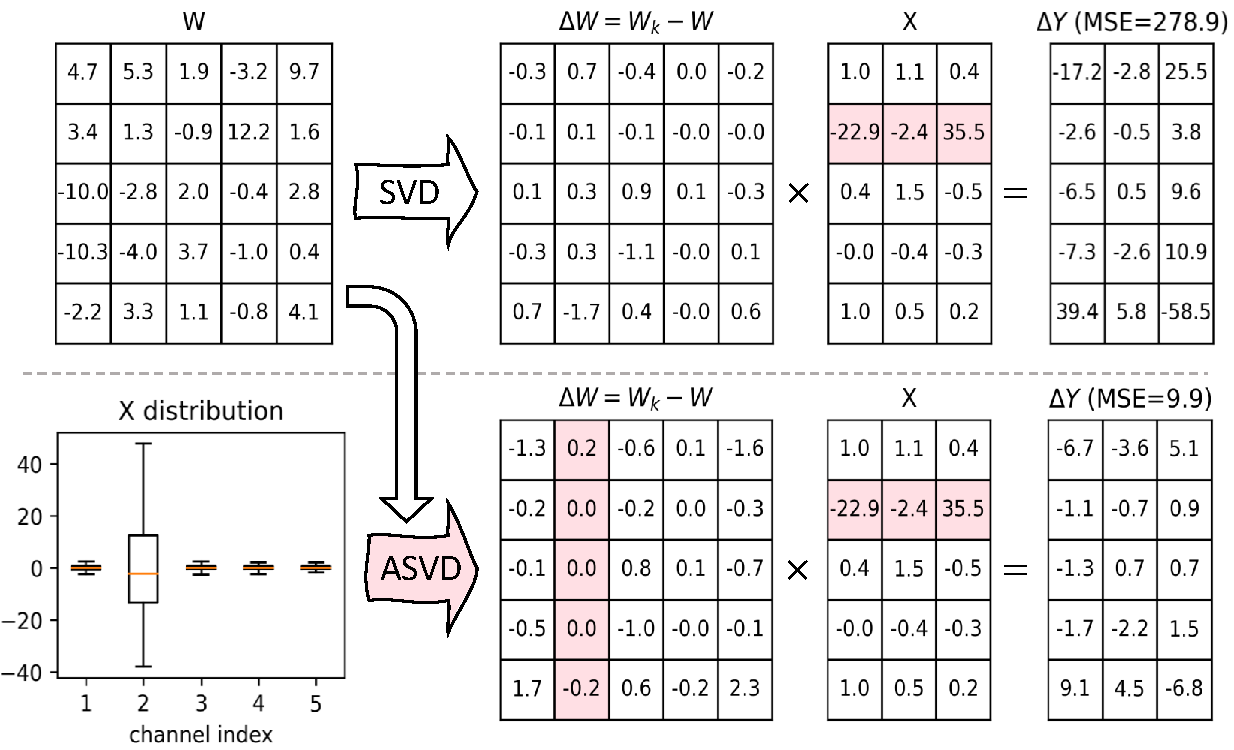
\includegraphics[width=0.8\textwidth]{ims/asvd_concept.pdf} %ims/xx.png
    \vspace{-0.1in}
    \caption{\small Comparison between SVD and \asvd. Outlier channels in input activations ($\mathbf{X}$) are highlight in red, and \asvd~takes these into consideration, which can contribute to a reduction in output error.}
    \label{im_svd_asvd_concept}
    \vspace{-0.2in}
\end{figure}

\textbf{Challenge 1: Influence of Activation}: 
% Recent studies in LLM post-training quantization~\cite{lin2023awq,wei2022outlier,wei2023outlier,frantar2022gptq} have underscored the importance of considering activations when compressing LLM weights. 
This perspective shifts the focus from solely relying on the truncation error $\mathbf{L}_{\text{t}}$, which depends only on the model's weights, to also accounting for the activations. The rationale behind this is the critical role of outliers in activations within LLMs ~\citep{lin2023awq,wei2022outlier,kim2023squeezellm}. Thus, for effective LLM decomposition, our objective optimization becomes:
\begin{equation}
\begin{aligned}
    \mathbf{W}_k^{\star} &= \arg\min_{\mathbf{W}_k}\Vert \mathbf{W}_k\mathbf{X} - \mathbf{W}\mathbf{X} \Vert_{F}^2.
\end{aligned}
\end{equation}
Here, $\mathbf{X}$ represents the input activations, which are cached from a small calibration set. This set is derived from the pre-training dataset to avoid overfitting to a specific task. 
Essentially, our objective is to ensure that the output of the decomposed LLM closely mimics the output of the original LLM, rather than merely aligning their weights. This approach prioritizes functional equivalence over structural similarity, recognizing that accurate output replication is more critical for maintaining the model's post-decomposition performance. 
We define the variation in activations between the compressed matrix $\mathbf{W}_k$ and the original matrix $\mathbf{W}$ as:
\begin{equation}
    \Delta\mathbf{Y} = (\mathbf{W}_k - \mathbf{W})\mathbf{X}. 
\label{eq:delta_y}
\end{equation}
To illustrate this concept, we visualize an example of $\mathbf{W}$, $\mathbf{W}_k$ (decomposed by simply SVD), $\mathbf{X}$, and the resulting variation in activations $\Delta\mathbf{Y}$ in Fig.~\ref{im_svd_asvd_concept} (Top line). This visualization reveals a critical insight: even when the variation in weights $\Delta\mathbf{W} = \mathbf{W} - \mathbf{W}_k$ is relatively minor, the corresponding variation in activations $\Delta\mathbf{Y}$ can be huge. This significant variation in activations is a key factor in why a straightforward SVD-based decomposition approach falls short in effectively decomposing LLMs. The activation variations, despite being derived from input activations of large magnitude (not the weight variations), can lead to considerable changes in the whole model's output, thereby undermining the decomposition's efficacy.

\textbf{Challenge 2: Singular Values Variations among Layers}: 
The distribution of singular values within a matrix is indicative of its sparsity and, by extension, its sensitivity to certain types of information~\citep{kim2015compression,kim2019efficient,wen2017coordinating}. In LLMs, there is a notable variation in singular values across different layers. 
Specifically, some layers exhibit a concentration of large singular values, signifying less sensitivity to weight variation. This characteristic often correlates with these layers being easy to compress. Conversely, other layers in the LLMs display a more uniform distribution of smaller singular values. Such a pattern suggests a balanced contribution from various singular vector pairs. This variability in the distribution of singular values among layers presents a unique challenge, as it implies that each layer may require a tailored approach to decompose and maintain the overall functionality of the LLM. 

These challenges underscore the necessity for innovative approaches specifically designed for the LLM decomposition. Our objective is to achieve efficient compression while circumventing the substantial computational and data demands associated with training-based methods. 
To address the first challenge, we introduce an Activation-aware SVD mechanism, which is detailed in Section \ref{sec:method-activation}. This method is designed to mitigate the impact of weight variation on activations. For the second challenge, we propose a Sensitivity-based Truncation Rank Searching mechanism, elaborated in Section \ref{sec:method-sensitivity}, which adapts to the varying singular value distributions among different layers. 
% These tailored strategies aim to ensure that the decompression maintains the functional integrity of the LLMs while optimizing the memory and computational efficiency.


\subsection{\asvd: Activation-aware Singular Value Decomposition}
\label{sec:method-activation}

\asvd~is designed to refine the weight matrix $\mathbf{W}$ in LLMs by taking into account the effect of input activation channels. The process comprises the following three steps:

\noindent\textbf{Transforming the Weight Matrix.} The first step involves transforming the weight matrix $\mathbf{W}$ into an invertible matrix $\mathbf{S}$. 
% This matrix $\mathbf{S}$ is constructed to represent the impact of input channels on the weights, essentially adjusting $\mathbf{W}$ to better adapt with the activation patterns of the input $\mathbf{X}$. 
The transform is denoted as $\mathbf{WS}$.
Because the matrix $\mathbf{S}$ is invertible, we can have this equation:
\begin{equation}
    \mathbf{W} = \mathbf{WSS}^{-1} = (\mathbf{WS})\mathbf{S}^{-1}.
\end{equation}
% The transform matrix $\mathbf{S}$ is constructed to adjust $\mathbf{W}$ to better adapt with the activation patterns of the input $\mathbf{X}$. 
% This scaling step is important, as it modifies the weight matrix to reflect the varying importance of different input activations, making the decomposition more effective and targeted.

\noindent\textbf{Applying SVD to the Transformed Matrix.} After transforming the weight matrix, the next step is to apply SVD to the transformed matrix $\mathbf{WS}$. The SVD of $\mathbf{WS}$ is expressed as $\mathbf{WS} = \mathbf{U}^{\prime}\mathbf{\Sigma}^{\prime}{\mathbf{V}^{\prime}}^{T}$. 
To reduce the elements in these matrices, we truncate them to retain only the top-$k$ singular values. The truncated form of the decomposition is represented as:
\begin{equation}
    \mathbf{WS} \approx \mathbf{U}_k^{\prime}\mathbf{\Sigma}_k^{\prime}{\mathbf{V}_k^{\prime}}^{T}.
\end{equation}
This step ensures that the most significant aspects of the scaled weight matrix are retained. While less critical information, which contributes minimally to the model's output, is discarded. 

\textbf{Reconstructing the Approximated Weight Matrix.} The final step is to reconstruct an approximation of the original weight matrix. 
We multiply ${\mathbf{V}_k^{\prime}}^T$ with $\mathbf{S}^{-1}$ to produce a new matrix ${\mathbf{V}_k^{\prime\prime}}^T$:
\begin{equation}
    {\mathbf{V}_k^{\prime\prime}}^T = {\mathbf{V}_k^{\prime}}^T \mathbf{S}^{-1}.
\end{equation}
Note that the matrix ${\mathbf{V}_k^{\prime\prime}}^T$ has the same shape as the matrix ${\mathbf{V}_k^{\prime}}^T$.
In this way, the weight matrix can be approximated by:
\begin{equation}
    \mathbf{W} = (\mathbf{WS})\mathbf{S}^{-1}
    \approx (\mathbf{U}_k^{\prime}\mathbf{\Sigma}_k^{\prime}{\mathbf{V}_k^{\prime}}^{T}) \mathbf{S}^{-1}  = \mathbf{U}_k^{\prime}\mathbf{\Sigma}_k^{\prime}{\mathbf{V}_k^{\prime\prime}}^T
    = \mathbf{W}_k.
\end{equation}

% \asvd~focus on channel-wise activation outliers, striving to mitigate these outliers by appropriately scaling the corresponding weights. In this way, the activation variation can be mitigated as illustrated in Fig.~\ref{im_svd_asvd_concept}. 
% Note that the diagonal nature of $\mathbf{S}$ simplifies its inversion process, making $\mathbf{S}^{-1}$ computationally efficient.
% The subsequent challenge is to devise a method or criteria for accurately determining $\mathbf{S}$ so that it effectively aligns with the activation patterns observed in the LLM, ensuring that the scaling process optimally addresses the outlier activations.


% The $i$-th diagonal element in matrix $\mathbf{S}$, denoted as $\mathbf{S}_{ii}$, plays a critical role in scaling the weight matrix $\mathbf{W}$ by reflecting the importance of the $i$-th input channel in the neural network. The significance of this element lies in its ability to modulate the influence of each channel on the weight adjustments during the training process as shown in Fig.\ref{im_svd_asvd_concept} (Bottom line). To determine the value of $\mathbf{S}_{ii}$, several methods are explored, each focusing on different aspects of input activation.
% $S_{ii}$ is pivotal in moduling the input channel as: $(WS)_{:,i}=W_{:,i}S_{ii}$

\noindent\textbf{Setting the Transform Matrix $\mathbf{S}$.} 
The transform matrix $\mathbf{S}$ is constructed to adjust $\mathbf{W}$ to better adapt with the activation patterns of the input $\mathbf{X}$.
A simple method is to set the transform matrix as a diagonal matrix.
The computation of the linear layer can be transformed by:
\begin{equation}
    \mathbf{W}\mathbf{X}
    = (\mathbf{WS})(\mathbf{S}^{-1}\mathbf{X}).
\end{equation}
Each diagonal element in the matrix $\mathbf{S}_{ii}$ transforms the $i$-th input channel of weight as: $(\mathbf{WS})_{:,i}=\mathbf{W}_{:,i}\mathbf{S}_{ii}$. Because $\mathbf{S}^{-1}$ is also a diagonal matrix, the $\mathbf{S}_{ii}^{-1}$ scales the $i$-th channel of the activation as $\mathbf{S}^{-1}_{ii}\mathbf{X}_{i,:}$. This scaling adjusts how each activation channel impacts the weight matrix during the decomposition process. We visualize the impact of the adjustment in Fig.\ref{im_svd_asvd_concept}.
We use a small number of corpus sent to the LLM and calculate the absolute mean value of input activation channel. Then we set $\mathbf{S}_{ii}$ according to the absolute mean value of the activations in the $i$-th channel: 
% $\mathbf{S}_{ii} = (\frac{1}{n} \sum_{j=1}^{n} |\mathbf{X}_{ij}|)^\alpha$,
\begin{equation}
\mathbf{S}_{ii} := (\frac{1}{n} \sum_{j=1}^{n} |\mathbf{X}_{ij}|)^\alpha,
\label{eq:set_matrix_magnitude}
\end{equation}
where $n$  is the total number of activations for the $i$-th channel and hyper-parameter $\alpha$ provides flexibility to adjust the level of activation sensitivity incorporated into the scaling. This method focuses on the average magnitude of activation in each channel, capturing the general intensity of activation signals regardless of their positive or negative nature. 
Since we only need to do the LLM inference several times, this method is very fast.

% Another method to set the transform matrix is to optimize the $\mathbf{S}$ to reduce the output error introduced by decomposition:
Another method to set the transform matrix $\mathbf{S}$ to is to optimize the output error introduced by decomposition directly:
$\arg\min_{\mathbf{S}}\Vert \Delta \mathbf{Y} \Vert_{F}^2$.
\citet{wang2024svdllm} demonstrate that this optimization problem has analytic expression by setting the $\mathbf{S}$ to a lower triangular matrix $\mathbf{L}$, where $\mathbf{L}$ is the Cholesky decomposition of $\mathbf{X}\mathbf{X}^T$:
\begin{equation}
    \mathbf{S}:= \mathbf{L},~~\text{where}~~
     \mathbf{L}\mathbf{L}^T= \mathbf{X}\mathbf{X}^T.
 \label{eq:set_matrix_cholosky}
\end{equation}
This method takes an additional step to execute the Cholesky decomposition~\citep{meyer2000cholesky}. Despite this extra computation, it results in a lower output error $\Delta \mathbf{Y}$.

By designing an invertible transformation matrix $\mathbf{S}$, we can transform the weight matrix $\mathbf{W}$ into a decomposition-friendly matrix $\mathbf{WS}$. This transformation takes into account both input and output activations, making the subsequent decomposition more effective for compression. This is so-called  Activation-aware Singular Value Decomposition (ASVD).



\subsection{Sensitivity-based Truncation Rank Searching}
\label{sec:method-sensitivity}

\begin{figure}[h] 
    \centering
    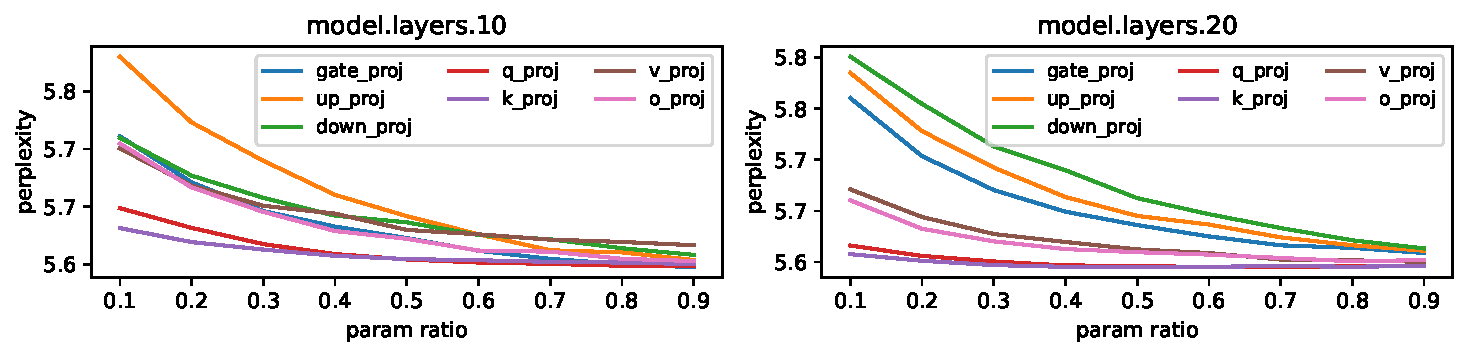
\includegraphics[width=0.95\textwidth]{ims/sensitivity.pdf} %ims/xx.png
    \vspace{-0.1in}
    \caption{Perplexity across Various Linear Layers and Parameter Ratios on LLaMA-2-7b.}
    \label{im_sensitivity}
    \vspace{-0.15in}
\end{figure}

% Targeting the second challenge, singular values variability among layers, we analyze the sensitivity of truncation ranking to the influence of prediction accuracy, and then set the truncation rank according to the sensitivity. We call this method as Sensitivity-based Truncation Rank Searching (STRS). 
The second challenge arises from the fact that different layers in LLMs exhibit varying degrees of sensitivity to information compression, which is reflected in the distribution of their singular values. 
Targeting this challenge, we propose the Sensitivity-based Truncation Rank Searching (STRS) method. 
STRS evaluates the layer sensitivity and decides the best truncation of singular values.
In the realm of NLP, perplexity is a key metric for assessing how effectively a language model predicts a sequence of tokens~\citep{brown2020language}. Therefore, we use the reduction in perplexity on the calibration dataset to evaluate the sensitivity of each layer. 
Similar to post-training compression methods~\citep{dettmers2022llm,frantar2022gptq,frantar2023sparsegpt}, we collect a small number of input token sequences as calibration dataset.

% At first, we collect a small calibration dataset. 
% This dataset serves as a component in evaluating the responsiveness of the layers to changes in truncation ranking. 
% To construct this calibration dataset, we sample some sequences from a source like Wikitext.
% Perplexity is a metric commonly used in natural language processing tasks to measure how well a language model predicts a given sequence of tokens. In our context, sensitivity is defined as the decreasing of perplexity observed on the sequences in the calibration dataset after decomposition.

% In the sensitivity evaluation process, an exploration of the neural network's response to varying truncation ratios is conducted. A set of potential parameter ratios is defined as $R$, including values such as 0.1, 0.2, ..., 0.9. These ratios control the proportion of rank $k$ retained during the SVD truncation on a weight with shape $m\times n$:



The core of the sensitivity evaluation process involves an in-depth exploration of how the neural network reacts to varying levels of truncation. We define a set of potential truncation ratios, denoted as $R=\{0.1, 0.2, \cdots, 0.9\}$. These ratios $r=\frac{km+kn}{mn}$ determine the fraction of the rank $k$ preserved during the SVD truncation for a weight matrix with dimensions $m\times n$. 
% \begin{equation}
%     r=\frac{km+kn}{mn}, r\in R.
% \end{equation}
For each linear layer in the LLM, we iterate through these candidate ratios. At each ratio, truncated SVD is applied to the layer's weight matrix, temporarily replacing the original layer in the model with this decomposed version. The model's perplexity is then evaluated on the calibration dataset.
% This iterative process allows us to determine the truncation ratio that optimally balances model compression with minimal impact on prediction accuracy.



This detailed exploration of sensitivity across various truncation levels provides essential insights into each layer's performance dynamics, informing the optimization and decision-making processes in model compression. As illustrated in Fig.~\ref{im_sensitivity}, there are noticeable variations in sensitivity among the different layers. Three key observations emerge from this analysis: 
1. Inversely Proportional Relationship: lower parameter ratios tend to result in higher perplexity scores. 
2. Higher Sensitivity in MLP Layers: MLP layers demonstrate higher sensitivity, indicating where more cautious truncation is necessary.
3. Variable Sensitivity Among Layers: Some layers exhibit relatively lower sensitivity, indicating potential for more aggressive compression. 
% These finding highlights the critical trade-off between model compression and reasoning performance, signaling the importance of careful parameter selection to maintain a balance. 
% This variation suggests the presence of redundancy within LLMs, presenting opportunities for more efficient compression approaches. Targeting these less-sensitive layers could lead to models that are both compact and computationally efficient.

% Post sensitivity evaluation, we compile a list of tuples (layer, truncation rank, sensitivity) and sort it according to sensitivity.
Assuming the affects of layers are independent, we should set the truncation rank of each layer to minimize the total affect to perplexity under the constraint of parameter size.
We propose a binary search algorithm to search for the best truncation rank.
Detailed explanations of algorithm can be found in the Appendix. 
% It designed to navigate the complexity of selecting the most effective truncation ranks for each layer, based on their sensitivity and contribution to the overall model performance. 

% \subsection{Absorbing Singular Values}
% \label{sec_efficeint_inference}

% After we decompose a matrix via \asvd, we can represent the weight matrix as a product of three matrices, i.e., $\mathbf{W} \approx \mathbf{U}_k \mathbf{\Sigma}_k \mathbf{V}_k^T$. 
% Thanks to the diagonal nature of matrix $\mathbf{\Sigma}_k$, we can further optimize the inference process. 
% Specifically, we can efficiently absorb the singular values in $\mathbf{\Sigma}_k$ into the matrices $U_k$ and $V_k^T$. We achieve this fusion using the following strategy: $\mathbf{A}_k = \mathbf{U}_k\sqrt{\mathbf{\Sigma}_k}$ and $\mathbf{B}_k = \sqrt{\mathbf{\Sigma}_k}\mathbf{V}_k^T$. Consequently, we obtain a more computationally efficient matrix operation~\footnote{See Appendix for details.}: 
% \begin{equation}
%     \mathbf{Y}=\mathbf{W}\mathbf{X} \approx \mathbf{A}_k (\mathbf{B}_k\mathbf{X})
% \end{equation}
% % Comparing with only fuse sigma into U or V, our proposed fusion method is benefit to quantization as shown in Table~\ref{tab_fusion}, as it can reduce the difference across different channels
% Compared to the methods of fusing the singular values $\mathbf{\Sigma}_k$ solely into either $\mathbf{U}$ or $\mathbf{V}$ matrices, our proposed fusion technique offers significant advantages in terms of weight quantization, as demonstrated in Table~\ref{tab_fusion}. Our approach involves evenly distributing the singular values from the diagonal matrix $\mathbf{\Sigma}_k$ into both $\mathbf{U}_k$ and $\mathbf{V}_k^T$ matrices. This ensures a more uniform distribution of $\mathbf{A}_k$ and $\mathbf{B}_k$, leading to a reduction in the disparity across different channels and reducing the quantization error.

% \begin{table}[t]
% \centering
% \caption{Perplexity on Wikitext-2 under different absorbing strategies after \asvd~on OPT-125m.}
% \label{tab_fusion}
% \resizebox{0.8\linewidth}{!}{
% \begin{tabular}{@{}cc@{\hspace{0.5em}}c@{\hspace{0.5em}}c@{\hspace{0.5em}}c@{}}
% \toprule
% param ratio & weight quant & absorbed by UV & absorbed by U & absorbed by V \\ \midrule
% 0.9         & INT6         & \textbf{37.58}      & 39.67     & 40.62     \\
% 0.85        & INT6         & \textbf{60.44}    & 64.19   & 61.02   \\ \bottomrule
% \end{tabular}
% }
% \vspace{-0.3in}
% \end{table}

\subsection{\asvd~for KV Cache Compression}

\begin{figure}[!h] 
    \centering
    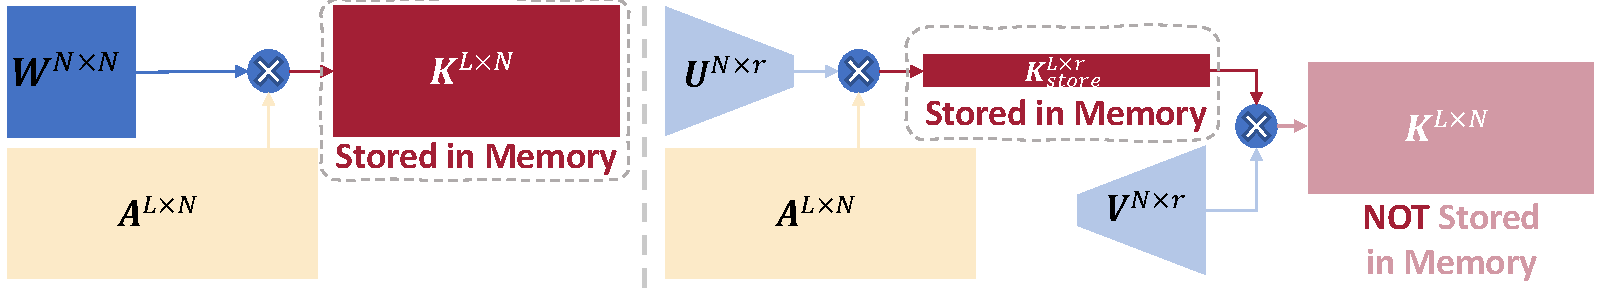
\includegraphics[width=0.98\textwidth]{ims/kvcompression-crop.pdf}
    \caption{\textbf{A demonstration of how \asvd~reduces the memory cost of the K cache.} \textbf{(Left)} With long text lengths $L$, the memory required for storing the K cache in a $N$-dimensional space becomes substantial. \textbf{(Right)} \asvd~decomposes the key projection weight matrix $\mathbf{W}$ into two low-rank matrices $\mathbf{U}$ and $\mathbf{V}$ (see Sec.~\ref{sec:method-activation}). This low-rank structure allows the K representation to be stored in a reduced $r$-dimensional space, where $r\ll N$. Consequently, we only need to save the intermediate K in the $r$ dimension instead of $N$ dimension, saving the K cache $\frac{N}{r}$ times. Note that saving V cache is the same, and when content length $L$ becomes really large (e.g., 1M tokens) or with larger batch size, the KV cache becomes a significant factor in memory cost.}
    \label{fig:kvcompression}
    \vspace{-0.2in}
\end{figure}


LLM inference with large context lengths can be incredibly resource-intensive, requiring high-end GPUs and, for the largest models, costly multi-GPU setups. Analysis of generative inference with LLMs reveals that, for relatively small batch sizes, the computation is primarily memory-bound \citep{hooper2024kvquant,liu2024tuning}. Given the growing gap between computational speeds and memory speeds, this issue is expected to worsen over time, making it crucial to address the memory bottleneck. Further analysis indicates that the memory bottleneck is strongly correlated with context size. For long sequence lengths, the main contributor to memory consumption is the KV cache storing, so minimizing the KV cache can reduce both memory consumption and bandwidth requirements \citep{yuan2024llmunveiled}.

As we discussed in Sec.\ref{sec:method-activation}, \asvd~decomposes the key and value projection weight matrix $\mathbf{W}\in \mathbb{R}^{N\times N}$ into two low-rank matrices, $\mathbf{U}\in \mathbb{R}^{N\times r}$ and $\mathbf{V}\in \mathbb{R}^{N\times r}$, in a training-free manner, where $N$ is the dimension of K/V embedding space.
As shown in Fig.\ref{fig:kvcompression}, replacing the high-rank matrix with two low-rank matrices via \asvd~allows us to obtain intermediate activations in low-rank form. These intermediate activations can be stored as a replacement for the original KV cache.
In other words, the original KV cache requires storing two $L\times N$ matrices. With \asvd, the new KV cache only needs to store two $L\times r$ matrices. 
In summary, \asvd~can compress the KV cache $\frac{N}{r}$ times.
This significant reduction in memory usage for the KV cache enables larger batch sizes or longer sequence lengths, which are critical for real-world applications.

% To effectively determine the values of $\mathbf{S}_{ii}$, various methodologies are explored. 
% Each of these methods focuses on different characteristics of input activation, aiming to optimize $\mathbf{S}$ so that it accurately reflects the importance and influence of each input channel. This exploration is crucial for ensuring that the scaling aligns with the activation patterns observed in the LLM, thereby enhancing the effectiveness of the \asvd~process.

% \textit{Absolute Mean Value of Input Activation}: This method calculates $\mathbf{S}_{ii}$ by calculating the absolute mean value of the activations in the $i$-th channel. Mathematically, if $\mathbf{X}_{i,:}$ represents the input activation values of the $i$-th channel, then $\mathbf{S}_{ii}$ is computed as: $\mathbf{S}_{ii} = (\frac{1}{n} \sum_{j=1}^{n} |\mathbf{X}_{ij}|)^\alpha$,
% % \begin{equation}
% % \mathbf{S}_{ii} = (\frac{1}{n} \sum_{j=1}^{n} |\mathbf{X}_{ij}|)^\alpha,
% % \end{equation}
% % \vspace{-0.1in}
% where $n$  is the total number of activations for the $i$-th channel and hyper-parameter $\alpha$ provides flexibility to adjust the level of activation sensitivity incorporated into the scaling. This method focuses on the average magnitude of activation in each channel, capturing the general intensity of activation signals irrespective of their positive or negative nature.


% \textit{Absolute Maximum Value of Input Activation}: Diverging from the mean-based approach, this method zeroes in on the peak activation within each channel. Under this approach, $\mathbf{S}_{ii}$ is determined by the highest absolute value observed in the activations of the $i$-th channel. The formal expression for this calculation is: $\mathbf{S}_{ii} = (\max_{j} (|\mathbf{X}_{ij}|))^\alpha$.
% % \begin{equation}
% % \mathbf{S}_{ii} = (\max_{j} (|\mathbf{X}_{ij}|))^\alpha.
% % \end{equation}
% This method places emphasis on the most significant, or peak, activation in each channel, positing it as a key indicator of the channel's overall impact and importance. By focusing on the peak values, this approach underscores the channels with the most pronounced activation responses, considering them as crucial contributors to the network's functionality.